\section{Results and Discussion}
\label{sec:results}
Tables~\ref{tab:level1}--\ref{tab:level3} report test scores by level. Each score is the mean over three seeds from one refit on the 930 development decisions.

% Three single-column tables, one per level. Numbers copied from improved_v1/all_conditions_test_v1/validation_test_comparison.csv.
\newcommand{\abhead}{%
    \toprule
    Model & Acc. & MCC & AUC & LL \\
    \midrule}

\begin{table}[t]
    \caption{Level 1 baselines. Test: 235 decisions, 0.583 majority rate. LL is log loss; last direction gives hard labels, so it has none.}
    \label{tab:level1}
    \centering
    \scriptsize
    \setlength{\tabcolsep}{4pt}
    \begin{tabular}{lcccc}
        \abhead
        Training majority & 0.583 & 0.000 & 0.500 & 0.681 \\
        Last direction & 0.540 & 0.049 & 0.519 & -- \\
        Market only & 0.552 & 0.000 & 0.500 & 0.689 \\
        Market + availability & 0.563 & 0.017 & 0.493 & 0.687 \\
        Market + FinBERT + availability & 0.583 & 0.000 & 0.499 & 0.684 \\
        Tuned market only & 0.590 & 0.080 & 0.510 & 0.682 \\
        \bottomrule
    \end{tabular}
\end{table}

\begin{table}[t]
    \caption{Level 2 text representations.}
    \label{tab:level2}
    \centering
    \scriptsize
    \setlength{\tabcolsep}{4pt}
    \begin{tabular}{lcccc}
        \abhead
        TF-IDF + SVD & 0.489 & $-$0.086 & 0.469 & 0.705 \\
        Word2Vec & 0.579 & $-$0.008 & 0.502 & 0.684 \\
        FinBERT & 0.583 & 0.000 & 0.499 & 0.684 \\
        RoBERTa-base & 0.583 & 0.000 & 0.500 & 0.685 \\
        FinBERT, text only & 0.583 & 0.000 & 0.494 & 0.682 \\
        \bottomrule
    \end{tabular}
\end{table}

\begin{table}[t]
    \caption{Level 3 fusion components added to FinBERT.}
    \label{tab:level3}
    \centering
    \scriptsize
    \setlength{\tabcolsep}{4pt}
    \begin{tabular}{lcccc}
        \abhead
        Mean pooling (FinBERT) & 0.583 & 0.000 & 0.499 & 0.684 \\
        + task query & 0.528 & 0.000 & 0.500 & 0.686 \\
        + cross-attention & 0.584 & 0.026 & 0.501 & 0.683 \\
        + gate & 0.584 & 0.026 & 0.490 & 0.684 \\
        + all three & 0.528 & 0.005 & 0.485 & 0.686 \\
        \bottomrule
    \end{tabular}
\end{table}


\subsection{Validation}
No model beats the training prior. The prior has a validation log loss of 0.694. The best score, 0.689, comes from a tuned market-only model, and every text model falls between 0.691 and 0.705. Validation MCC stays between $-$0.009 and 0.077 for text models. TF-IDF with SVD has the highest value, 0.077, but also the worst log loss, 0.705. The success gate, which asks for a lower log loss than the prior in two folds, was not met. We wrote this gate after earlier test exposure, so it is not a true preregistration. FinBERT was selected for Level~3 because its mean log loss was lowest by less than 0.0002 over RoBERTa and the text-only model, so the choice carries little information.

\subsection{Test}
Test scores stay near chance. MCC ranges from $-$0.086 (TF-IDF with SVD) to 0.080, and the 0.080 belongs to the tuned market-only model, which sees no text. Four models (the majority baseline, FinBERT concatenation, RoBERTa, and the text-only FinBERT model) have MCC 0.000 and accuracy 0.583, equal to the share of UP days. They predict UP on all 235 days in every seed. Accuracy here reflects class balance in this period, not skill.

Paired intervals for MCC and log loss include zero for the contrasts we report. The difference in MCC between FinBERT concatenation and market only is $-$0.086 to 0.081 (95\% interval), and against market plus availability it is $-$0.113 to 0.072. Among Level~3 variants, cross-attention against mean pooling gives an MCC difference of 0.000 to 0.046 and a log-loss difference of $-$0.005 to 0.003. Some macro-F1 contrasts at Level~1 lie entirely below zero, but they reflect constant predictions, not a gain. The task query and full fusion are slightly worse than mean pooling in accuracy. The intervals are conditional on the fitted models, and the test period has been used by earlier experiments. We read them as descriptive and claim no component effect. The last-direction rule reaches MCC 0.049, but its interval, $-$0.074 to 0.159, also includes zero.

News content does not add information. FinBERT concatenation has MCC 0.000 and log loss 0.684, against 0.000 and 0.689 for market only and 0.017 and 0.687 for market plus availability, and the training prior, 0.681, is lower than all of them. No representation is best: FinBERT, RoBERTa, and Word2Vec all sit at chance (AUC 0.499 to 0.502), and TF-IDF with SVD is worst. The Level~3 components do not help either. Cross-attention and the gate reach MCC 0.026 against 0.000 for mean pooling, but log loss differs by at most 0.001 and AUC does not rise (0.501 and 0.490 against 0.499). The MCC gains are small, so we read them as descriptive only.

The gap between validation and test is largest for TF-IDF with SVD, from 0.077 to $-$0.086. Checkpoint selection on small 158-row folds may inflate validation scores. We did not test this.

\subsection{Error analysis}
\emph{Do the models make real predictions?} Fig.~\ref{fig:err-share} shows the share of test days each seed predicts UP. A bar at 1.0 means UP on every day, which equals the majority rule. The concatenation model does this in every seed. Full fusion differs by seed: seeds 42 and 123 predict UP almost always and seed 2026 predicts DOWN on every day, which averages to the 0.528 accuracy in Table~\ref{tab:level3}. A collapsed model scores at chance whatever the text contains.

% Generated by eda-visualization/make_error_figures.py
\begin{figure}[!t]
    \centering
    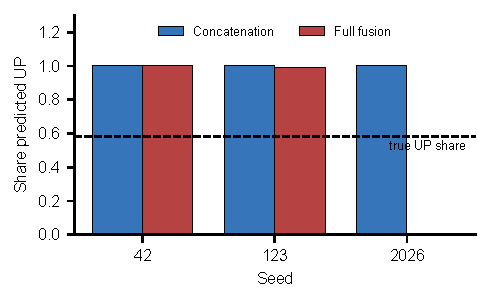
\includegraphics[width=\columnwidth]{err_up_share}
    \caption{Share of test days each model predicts UP, by seed. A bar at 1.0 means UP on every day. Dashed line: true UP share.}
    \label{fig:err-share}
\end{figure}


\emph{Is the signal missing, or can the model not read it?} A linear probe predicts a target from the day-average embedding. In Table~\ref{tab:probe}, the first four rows are an easy control: whether a day's titles have an above-median share of conflict, energy, rates, or China keywords. The probe reaches AUC 0.76--0.90, so the embeddings do carry topical content. The same probe predicts next-fixing direction at 0.46--0.50, inside the range of shuffled labels, although RoBERTa at 0.46 sits at its lower edge. The control labels come from the same titles, so they check the pipeline, not understanding. Fig.~\ref{fig:err-pca} shows the same vectors in two dimensions, coloured by direction. UP and DOWN days overlap almost completely, so direction is not visible even along the main variation of the text.

% Generated from eda-visualization/make_probe_table.py (development days only).
\begin{table}[t]
\centering
\caption{Linear probe AUC (L2 logistic regression, five time-ordered folds on 930 development days) on day-mean vectors. Random: Gaussian vectors of the same size. Shuffled: direction permuted in blocks of ten, 100 runs.}
\label{tab:probe}
\scriptsize
\setlength{\tabcolsep}{4pt}
\begin{tabular}{lcccc}
\toprule
Target & FinBERT & RoBERTa & W2V & Random \\
\midrule
Keyword: conflict & 0.88 & 0.86 & 0.88 & 0.49 \\
Keyword: energy & 0.84 & 0.87 & 0.87 & 0.49 \\
Keyword: rates/Fed & 0.88 & 0.89 & 0.90 & 0.51 \\
Keyword: China & 0.78 & 0.76 & 0.77 & 0.49 \\
\midrule
Direction (UP/DOWN) & 0.49 & 0.46 & 0.50 & 0.53 \\
Shuffled direction & 0.50 & 0.50 & 0.50 & 0.50 \\
\quad 95\% range & .45--.54 & .46--.53 & .46--.53 & .46--.54 \\
\bottomrule
\end{tabular}
\end{table}

% Generated by eda-visualization/make_error_figures.py
\begin{figure}[!t]
    \centering
    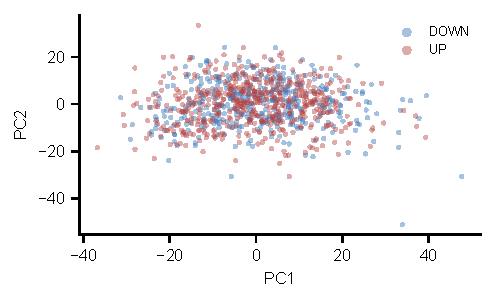
\includegraphics[width=\columnwidth]{err_pca}
    \caption{PCA of day-mean FinBERT vectors on development days, coloured by next-fixing direction. Heavy overlap means direction is not visible in the text vectors.}
    \label{fig:err-pca}
\end{figure}


\emph{Does attention find the informative articles?} Fig.~\ref{fig:err-attn} shows the weights on the largest false-UP day, the day where a useful signal would matter most. A value of 1 means an article gets the same weight as under plain averaging. Task-query weights are nearly uniform, and cross-attention is only mildly peaked, with no article standing out. The fusion behaves like mean pooling. The weights are descriptive, not causal, and they come from the test period.

% Generated by eda-visualization/make_error_figures.py
\begin{figure}[!t]
    \centering
    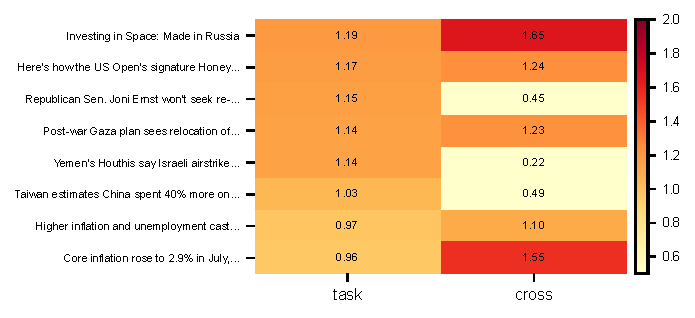
\includegraphics[width=\columnwidth]{err_attention_example}
    \caption{Attention on 2025-09-01, the largest false-UP day (14 articles). Values are weight divided by uniform weight, so 1 means equal weight. Columns: task query and cross-attention. Rows: the eight largest-weight articles of 14.}
    \label{fig:err-attn}
\end{figure}


\emph{Does news relate to returns at other times?} Fig.~\ref{fig:leadlag} correlates each daily news feature with the return $k$ days later, on development days only. If news led the market, bars at $k>0$ would leave the grey band, which marks what shifted copies of the news series produce by chance. Three of 66 correlations leave it, no more than chance allows. The one plausible case is that more articles appear on volatile days, which explains about 1.6\% of the variance and says nothing about direction.

% Generated by eda-visualization/make_leadlag.py (development days only).
\begin{figure}[!t]
    \centering
    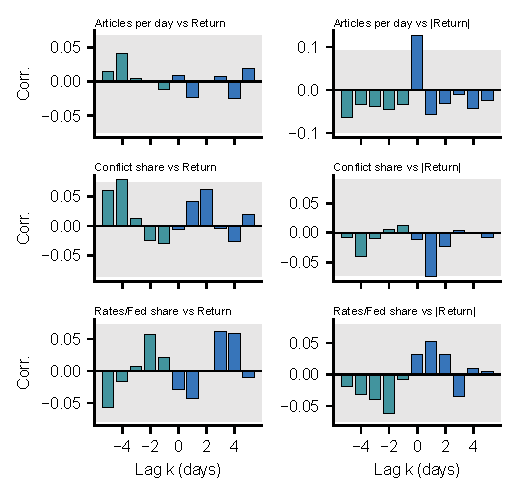
\includegraphics[width=\columnwidth]{lead_lag}
    \caption{Lead-lag correlation of news features with USD/IDR returns. Bars: correlation between a daily news feature and the return $k$ days later. Lag $k>0$: news leads. Grey band: widest 95\% range of circular-shift nulls across lags, a conservative envelope.}
    \label{fig:leadlag}
\end{figure}


\emph{Would more data help?} Fig.~\ref{fig:learning} trains the probe on a growing number of days and scores it on validation days. The keyword control, an easy target, rises to AUC 0.84 by 400 days. Direction stays between 0.43 and 0.55 at every training size and PCA dimension we tried (2 to 200), inside the grey chance band. In these features and this sample, more data does not reveal a direction signal.

% Generated by eda-visualization/make_learning_curve.py (train and validation days only).
\begin{figure}[!t]
    \centering
    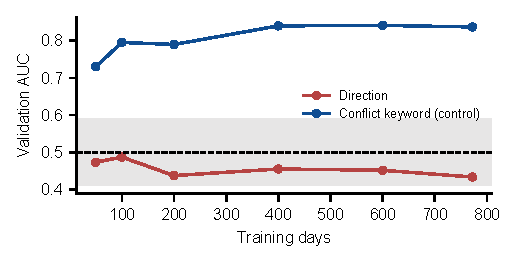
\includegraphics[width=\columnwidth]{learning_curve}
    \caption{Linear probe on FinBERT day means, scored on the 158 validation days, by training size. The keyword target is an easy control. Grey band: approximate 95\% null range of AUC ($\pm0.09$).}
    \label{fig:learning}
\end{figure}



\subsection{Limitations}
The 930 development decisions are the effective sample, not the 16{,}723 articles, because all articles of a day share one label. The test period was opened for the original corpus on 2026-11-11 and for the combined corpus on 2026-11-15. The improved\_v1 conditions were scored on it on 2026-11-16, after the log-loss selection rule replaced an earlier MCC-based Word2Vec choice, and later checks reused it. It is not an untouched holdout. News dates carry no time of day, article versions are unknown, and the encoders are frozen. We test one corpus and one horizon, and we measure direction, not trading return. These limits restrict the conclusion to this setup. They do not show that news carries no information about USD/IDR.
